\chapter{Background}
\label{cha:relatedwork}

In this section, the global system known as \emph{devices cloud} will be first detailed. Afterwards, the different possible technologies that could be used in this thesis will be introduced. Finally, an overview of the different researches and studies that have been previously performed will be given.
 
\section{The Devices Cloud}
Integrating the requirements defined in the Introduction to a more detailed view of the global system, the Figure \ref{fig:design_complete} of the \emph{devices cloud} architecture . Of course, only the information relevant for this thesis is depicted.

\begin{figure}[!ht]
	\centering
	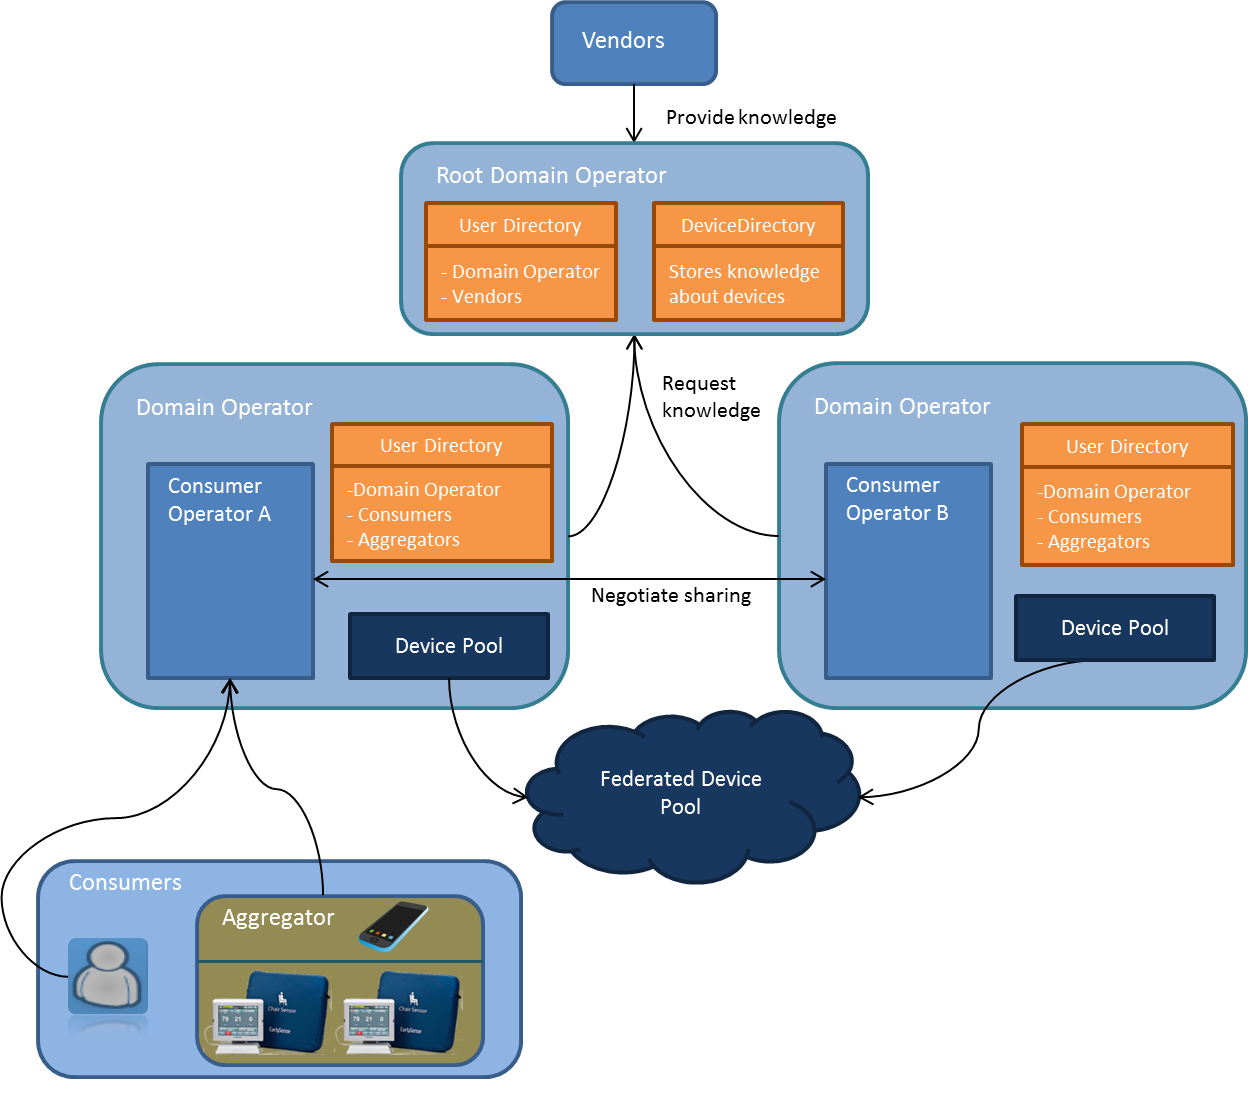
\includegraphics[scale=0.6]{images/design_complete}
	\caption{Detailed Architecture of the Devices Cloud}
	\label{fig:design_complete}
\end{figure}

\section{Authentication}
\subsection{Authentication from symmetric key}
\subsection{Authentication from asymmetric keys}
\subsection{Authentication from one-way function}
\subsection{Federated Identity Management}
\subsubsection{Kerberos}
\subsubsection{SAML}
\subsubsection{OpenId Connect}

\section{Related work}